\documentclass[11pt, oneside]{article}   	% use "amsart" instead of "article" for AMSLaTeX format
\usepackage{geometry}                		% See geometry.pdf to learn the layout options. There are lots.
\geometry{letterpaper}                   		% ... or a4paper or a5paper or ... 
%\geometry{landscape}                		% Activate for for rotated page geometry
%\usepackage[parfill]{parskip}    		% Activate to begin paragraphs with an empty line rather than an indent
\usepackage{graphicx}				% Use pdf, png, jpg, or eps§ with pdflatex; use eps in DVI mode
								% TeX will automatically convert eps --> pdf in pdflatex		
\usepackage{amssymb}
\usepackage[utf8]{inputenc}
\usepackage{listings}
\usepackage{enumitem}
\usepackage{hyperref}
\usepackage{anyfontsize}
\usepackage{tikz}
\usetikzlibrary{patterns,calc}

\newcommand{\sch}{\lstinline{tpl_sc_handler}}

\title{MSP430X port - small memory model version}
\author{Jean-Luc Béchennec, Mikaël Briday}
%\date{}							% Activate to display a given date or no date

\lstset{% general command to set parameter(s)
	basicstyle=\footnotesize\ttfamily,
	backgroundcolor=\color{lightgray!30},
	frame=single, framerule=0pt
}

\begin{document}
\maketitle

This document describes the small version for the CPUX of the Trampoline port on MSP430, which assumes that the code is hosted in the first 64kB of memory and therefore the addresses are stored on 16-bit words. Instruction set of the MSP430X is available in \cite{slau208q} or \cite{slau367o}.

\section{Multitasking}

\subsection{ABI}

In \cite{slaa664} a change has been made in GCC so that it conforms to the ABI defined in \cite{slaa534} and becomes compatible with the proprietary Texas Instruments compiler. So there are two GCC compilers for MSP430: the one that does not conform to the ABI defined by Texas Instruments, \emph{MSPGCC}, and the one that does conform to the ABI, \emph{GCC compiler for MSP}. 

As it is difficult to support both ABIs simultaneously, it was decided to support both ABIs at compile time. A precompiled \emph{MSPGCC} is available in the latest version of Energia\footnote{GCC 4.6.3.}. Energia can be downloaded at {\small\url{https://energia.nu}}. A precompiled \emph{GCC compiler for MSP} is available at {\small\url{http://www.ti.com/tool/msp430-gcc-opensource}}.

In both ABIs the registers used to pass arguments to functions are \lstinline{r12}, \lstinline{r13}, \lstinline{r14} and \lstinline{r15}. In the ABI of \emph{MSPGCC}, \lstinline{r15} is the first argument, \lstinline{r14} the second and so on. If a function returns a value, it is placed in \lstinline{r15}. In the ABI of \emph{GCC compiler for MSP} \lstinline{r12} is the first argument, \lstinline{r13} the second and so on. If a function returns a value, it is placed in \lstinline{r12}.
 No Trampoline service uses more than 3 arguments and therefore \lstinline{r12}, for \emph{MSPGCC} ABI, or \lstinline{r15}, for \emph{GCC compiler for MSP} ABI, is available to pass the service ID into the wrapper.
 
Adapting to both ABIs at compile time is not very complicated. This involves exchanging the use made of the registers \lstinline{r12}, identifying the service, and \lstinline{r15}, the return value of the service and the argument of \lstinline{tpl_run_elected}. This can be done by defining an abstract register to pass the service identifier and an abstract register to return the return value of the service. The register selection can be made using the preprocessor and the macro \lstinline{__GXX_ABI_VERSION} as shown at Figure \ref{lst:macroabi}. This macro is \lstinline{1002} for \emph{MSPGCC} and \lstinline{1011} for \emph{GCC compiler for MSP}. 2 abstract registers are defined: \lstinline{REG_SID} which is \lstinline{r12} in \emph{MSPGCC} ABI and \lstinline{r15} in \emph{GCC compiler for MSP} ABI, and \lstinline{REG_RETARG} which is \lstinline{r15} in \emph{MSPGCC} ABI and \lstinline{r12}  in \emph{GCC compiler for MSP} ABI.

\begin{figure}[h]
\caption{ABI selection with C preprocessor macros}
\begin{lstlisting}
#if __GXX_ABI_VERSION == 1002
/* MSPGCC ABI */
#define MSPGCC_ABI
#define REG_SID r12
#define REG_RETARG r15
#define REG_RETARG_OFFSET 8
#elif __GXX_ABI_VERSION == 1011
/* GCC compiler for MSP ABI */
#define GCCFORMSP_ABI
#define REG_SID r15
#define REG_RETARG r12
#define REG_RETARG_OFFSET 2
#else
#error "Unsupported ABI"
#endif
\end{lstlisting}
\label{lst:macroabi}
\end{figure}

The following table summarizes the use of the registers in both ABIs if we consider all arguments are small enough to be stored in one register. Although \lstinline{r11} is volatile in one of them, for simplification purposes later on, \lstinline{r11} is considered as non-volatile. A preserved register is noted P and a Volatile register is noted V.

\begin{center}
\begin{tabular}{|l|c|c|}
\hline
Register & \emph{MSPGCC} & \emph{GCC compiler for MSP} \\
\hline
\hline
\lstinline|r0| & \multicolumn{2}{c|}{Program Counter, saved on stack by cpu} \\
\hline
\lstinline|r1| & \multicolumn{2}{c|}{Stack Pointer} \\
\hline
\lstinline|r2| & \multicolumn{2}{c|}{Status Register} \\
\hline
\lstinline|r3| & \multicolumn{2}{c|}{Constants Generator} \\
\hline
\lstinline|r4-r10| & \multicolumn{2}{c|}{Not preserved by the callee} \\
\hline
\lstinline|r11| & V & P \\
\hline
\lstinline|r12| & V, argument 4 & V, argument 1, return value \\
\hline
\lstinline|r13| & V, argument 3 & V, argument 2 \\
\hline
\lstinline|r14| & V, argument 2 & V, argument 3 \\
\hline
\lstinline|r15| & V, argument 1, return value & V, argument 4 \\
\hline
\end{tabular}
\end{center}


It can be noted that the arguments being passed through the low weight 16 bits of the registers, except perhaps for the far pointers, the arguments of the Trampoline services must fit on 16 bits. This limits the tick argument of the services related to alarms to 16 bits. 

% Some Trampoline services use a pointer as an argument: \lstinline{GetTaskId}, \lstinline{GetTaskState}, \lstinline{GetAlarmBase}, \lstinline{GetAlarm}, \lstinline{GetEvent}, \lstinline{SendMessage}, \lstinline{ReceiveMessage}, \lstinline{GetCounterValue}, \lstinline{GetScheduleTableStatus} and \lstinline{GetApplica-}    \lstinline{tionState}. Since none of these services uses more than 2 arguments, a pointer to a high address will occupy 2 registers and the other argument only one. An AUTOSAR service is a problem: \lstinline{GetElapsedCounterValue}. This service takes 3 arguments, two of which are pointers. If the pointed data are in high addresses, some of the arguments will be passed through the stack. However, by forcing the storage of application data whose pointers have been passed to the OS in the lower memory, only 3 registers will be used. Not doing so would lead to unreasonable complexity of wrappers and of the services handler.

\subsection{Stack}
%\subsection{}

A service call is done using the \lstinline{br} instruction in the service call wrapper to prevent 2 nested call and fold the \lstinline{ret} instruction. The service identifier is passed to the service call handler through the \lstinline{REG_SID} register. So a service call wrapper is as shown in listing at figure \ref{lst:wrapper}.

\begin{figure}[h]
\caption{Service wrapper}
\begin{lstlisting}
    mov  #<service_id>, REG_SID /* put the service id in the ad-hoc reg */
    br   #tpl_sc_handler        /* branch to the service call handler   */
\end{lstlisting}
\label{lst:wrapper}
\end{figure}

When in the \sch\ the stack is as shown at figure \ref{fig:stacksc}\footnote{stacks are drawn with the lower address up so they are growing upward, not downward. Each stack location is a 16 bits word.}. \texttt{PTOS} stands for \emph{Process Top Of Stack}.

\begin{figure}[h]
\caption{Stack at beginning of \sch}
\centering
\vspace{1em}
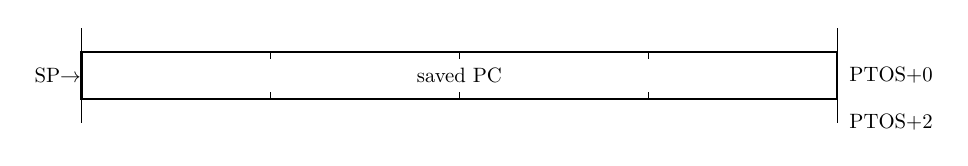
\begin{tikzpicture}[scale=0.6, every node/.style={scale=0.75}]
\draw[thick] (0,3) rectangle ++(16,1); \node at (8,3.5) {saved PC};
\foreach \x in {4,8,12} { \draw (\x,3) -- ++(0,.15);  \draw (\x,4) -- ++(0,-.15); }
%\draw[thick] (0,2) rectangle ++(16,1); \node at (14,2.5) {saved PC [19..16]};
%\draw[thick] (0,1) rectangle ++(16,1); \node at (8,1.5) {service identifier};
%\foreach \x in {4,8,12} { \draw (\x,1) -- ++(0,.15);  \draw (\x,2) -- ++(0,-.15); }
%\draw[thick] (0,0) rectangle ++(16,1); \node at (14,.5) {saved r11 [19..16]};
%\draw (12,0) -- ++(0,1);
%\draw[pattern=north west lines, pattern color=purple] (0,0) rectangle ++(12,1);
%\draw[pattern=north west lines, pattern color=purple] (0,2) rectangle ++(12,1);
\foreach \x in {0,16} \draw (\x,2.5) -- (\x,4.5);
\node at (-.5,3.5) {SP$\rightarrow$};
\foreach \y/\offset in {3.5/0,2.5/2} \node[anchor=west] at (16.1,\y) {PTOS+\offset};
\end{tikzpicture}
\label{fig:stacksc}
\end{figure}

When an interrupt is taken into account, the \lstinline{PC} and the \lstinline{SR} are pushed on the stack. To save space, the \lstinline{SR} is stored in the same 16-bit word as bits 19..16 of \lstinline{PC}. For an obscure reason, words are in reverse order and bits 19..16 of \lstinline{PC} are in high bits. Since all the code is in the first 64kb of the memory, bits 19 to 16 of the PC are always 0. The stack is shown at figure \ref{fig:stackit}.

\begin{figure}[h]
\caption{Stack in an interrupt handler}
\centering
\vspace{1em}
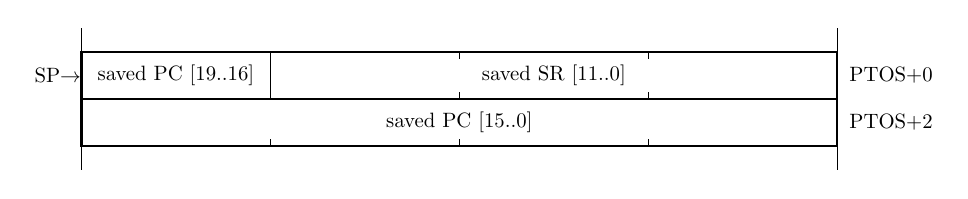
\begin{tikzpicture}[scale=0.6, every node/.style={scale=0.75}]
\draw[thick] (0,2) rectangle ++(16,1); \node at (8,2.5) {saved PC [15..0]};
\foreach \x in {4,8,12} { \draw (\x,2) -- ++(0,.15);  \draw (\x,4) -- ++(0,-.15); }
\draw[thick] (0,3) rectangle ++(16,1); \node at (2,3.5) {saved PC [19..16]}; \node at (10,3.5) {saved SR [11..0]};
\foreach \x in {4,8,12} { \draw (\x,3) -- ++(0,.15);  \draw (\x,4) -- ++(0,-.15); }
%\draw[thick] (0,1) rectangle ++(16,1); \node at (8,1.5) {saved r11 [15..0]};
%\foreach \x in {4,8,12} { \draw (\x,1) -- ++(0,.15);  \draw (\x,2) -- ++(0,-.15); }
%\draw[thick] (0,0) rectangle ++(16,1); \node at (14,.5) {saved r11 [19..16]};
\draw (4,3) -- ++(0,1);
%\draw[pattern=north west lines, pattern color=purple] (0,0) rectangle ++(12,1);
%\draw[pattern=north west lines, pattern color=purple] (0,2) rectangle ++(12,1);
\foreach \x in {0,16} \draw (\x,1.5) -- (\x,4.5);
\node at (-.5,3.5) {SP$\rightarrow$};
\foreach \y/\offset in {3.5/0,2.5/2} \node[anchor=west] at (16.1,\y) {PTOS+\offset};
\end{tikzpicture}
\label{fig:stackit}
\end{figure}

\subsubsection*{Preemption cases}

A preemption can be synchronous or asynchronous. A synchronous preemption (SP) happens when a service call is done, for instance when a task activates a higher priority task. An asynchronous preemption (AP) happens under interrupt, for instance when a higher priority task is activated by an alarm. A preempted task may resume its execution following a synchronous event (SR) : the running task calls \lstinline{TerminateTask}, \lstinline{ChainTask}, \lstinline{WaitEvent} or \lstinline{SetEvent} or following an asynchronous event (AR) : an alarm does a \lstinline{SetEvent}. So there are 4 cases:.

\begin{description}

\item[SPSR] Synchronous Preemption, Synchronous Resume. $\tau_1$ is running, $\tau_2$ is ready. $P(\tau_1) > P(\tau_2)$.
$\tau_1$ calls \lstinline{WaitEvent} and is preempted synchronously, $\tau_2$ becomes running and  calls \lstinline{SetEvent}. $\tau_2$ is preempted and $\tau_1$ is resumed synchronously.

\item[SPAR] Synchronous Preemption, Asynchronous Resume. $\tau_1$ calls \lstinline{WaitEvent} ans is synchronously preempted, An alarm does a \lstinline{SetEvent} on $\tau_1$ which is asynchronously resumed.

\item[APSR] Asynchronous Preemption, Synchronous Resume. $\tau_1$ is running, $\tau_2$ is suspended. $P(\tau_1) < P(\tau_2)$. An alarm activates $\tau_2$, $\tau_1$ is asynchronously preempted, $\tau_2$ calls \lstinline{TerminateTask}, $\tau_1$ is synchronously resumed.

\item[APAR] Asynchronous Preemption, Asynchronous Resume. $\tau_1$ is running, $\tau_2$ is suspended. $P(\tau_1) < P(\tau_2)$. An alarm activates $\tau_2$, $\tau_1$ is asynchronously preempted. $\tau_2$ is terminated by the OS because of protection fault, for instance a timing protection interrupt and $\tau_1$ is asynchronously resumed.

\end{description}

So \emph{the stack frame has to be normalized}. The normalized stack frame is the asynchronous one shown at figure \ref{fig:stackit} because it contains the Status Register. Normalization is done at the beginning of the \sch. The end of the \sch is done using the \texttt{reti} instruction, as at the end of an interrupt.

The normalized stack frame may be done only when a context is saved to prevent a normalization if there is no context switch. However, the load of the context is much complicated, as the restauration of \texttt{r2} (aka status register) in the \sch re-enable the interrupts before the end of the function.

\subsection{The tpl\_sc\_handler}

The background color of the code snippets depends on the current active stack:
\begin{description}
	\item[green] process stack
	\item[red]   kernel stack
	\item[yellow] either kernel or process stack
\end{description}

%\fbox{\parbox{.99\textwidth}{The stack structure should be reviewed for the \lstinline{tpl_sc_handler}. Since volatile registers must be stacked first by an ISR, they should be at the bottom of the stack, just above the PC, and not at the top.}}

\vspace{1em}

The first thing to do is to compare the service id to the number of services to verify its validity.

\begin{lstlisting}[backgroundcolor=\color{yellow!15}]
    cmp   #SYSCALL_COUNT, REG_SID
    jlo   tpl_sc_handler_id_ok                /* continue if lower        */
    ret                                       /* return if higher or same */
tpl_sc_handler_id_ok:
\end{lstlisting}

Disable interrupts so that the kernel cannot be interrupted. Check the reentrancy flag. If it is not zero, it means the service is called from a hook and has to be processed differently.

\begin{lstlisting}[backgroundcolor=\color{yellow!15}]
    dint
    tst.b &tpl_reentrancy_flag
    jnz   tpl_sc_handler_from_hook
\end{lstlisting}


We need to have the same stack pattern for both the \sch\ and an interrupt handler which calls the operating system. So we push the SR
 and we reset the 4 higher bits (high weight of PC, not sure it is needed)
 and set GIE in the saved SR.

\begin{lstlisting}[backgroundcolor=\color{yellow!15}]
    push         sr
    bic.b        #0xF0, 1(sp)     /* reset the 4 higher bits of saved SR */
    bis.b        #0x08, 0(sp)     /* set the GIE bit in the saved SR     */
\end{lstlisting}

The stack is then as follow:

\begin{center}
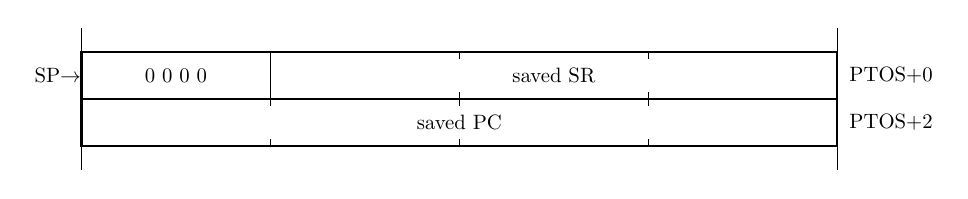
\begin{tikzpicture}[xscale=0.6,yscale=-0.6, every node/.style={scale=0.75}]
\draw[thick] (0,1) rectangle ++(16,1); \node at (8,1.5) {saved PC};
\draw[thick] (0,0) rectangle ++(16,1); \node at (10,0.5) {saved SR}; \node at (2,0.5) {0 0 0 0};
\draw (4,0) -- ++(0,1);
\foreach \y in {0,1} {
	\foreach \x in {4,8,12} { \draw (\x,\y) -- ++(0,.15);  \draw ($(\x,\y+1)$) -- ++(0,-.15); }
}
%\draw[thick] (0,2) rectangle ++(16,1); \node at (14,2.5) {saved PC [19..16]};
%\draw[thick] (0,1) rectangle ++(16,1); \node at (8,1.5) {service identifier};
%\foreach \x in {4,8,12} { \draw (\x,1) -- ++(0,.15);  \draw (\x,2) -- ++(0,-.15); }
%\draw[thick] (0,0) rectangle ++(16,1); \node at (14,.5) {saved r11 [19..16]};
%\draw (12,0) -- ++(0,1);
%\draw[pattern=north west lines, pattern color=purple] (0,0) rectangle ++(12,1);
%\draw[pattern=north west lines, pattern color=purple] (0,2) rectangle ++(12,1);
\foreach \x in {0,16} \draw (\x,-0.5) -- (\x,2.5);
\node at (-.5,0.5) {SP$\rightarrow$};
\foreach \offset in {0,2} \node[anchor=west] at ($(16.1,.5+.5*\offset)$) {PTOS+\offset};
\end{tikzpicture}
\end{center}

Obviously volatile registers (r12 to r15 because we take into account both ABIs) are not saved in \sch\ since the caller does not expect their values to be preserved but we need to make room (8 bytes) on the stack for them because an interrupt handler will save these registers at this location. However register names appear in figures but are in italic. Either \textit{r12} if MSPGCC ABI is used or \textit{r15} if GCC for MSP ABI is used is for the \lstinline{REG_RETARG} which is not saved yet.

\begin{lstlisting}[backgroundcolor=\color{yellow!15}]
    sub  #8, sp
\end{lstlisting}

The \sch\ needs one working register and we choose to use \lstinline{r11} which has to be saved on the process stack before using it.

\begin{lstlisting}[backgroundcolor=\color{yellow!15}]
    push r11
\end{lstlisting}

At that stage the stack is shown in figure \ref{fig:stackShapeBeforeCallingService}.

\begin{figure}[t]
\caption{Stack shape before calling the service}
\begin{center}
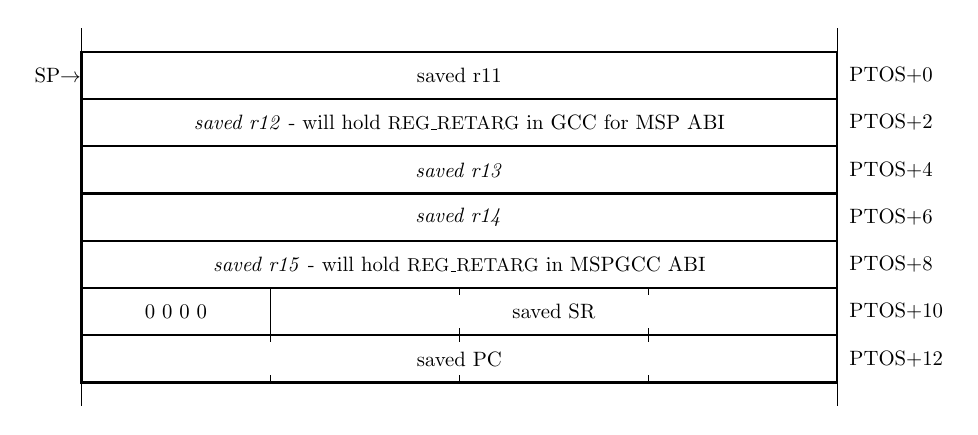
\begin{tikzpicture}[xscale=0.6, yscale=-.6, every node/.style={scale=0.75}]
\draw[thick] (0,0) rectangle ++(16,1); \node at (8,0.5) {saved r11};
\draw[thick] (0,6) rectangle ++(16,1); \node at (8,6.5) {saved PC};
\draw[thick] (0,5) rectangle ++(16,1); \node at (10,5.5) {saved SR}; \node at (2,5.5) {0 0 0 0};
\draw (4,5) -- ++(0,1);
\foreach \y in {5,6} {
	\foreach \x in {4,8,12} { \draw (\x,\y) -- ++(0,.15);  \draw ($(\x,\y+1)$) -- ++(0,-.15); }
}
%\draw[thick] (0,5) rectangle ++(16,1); \node at (8,5.5) {saved PC [15..0]};
%\foreach \x in {4,8,12} { \draw (\x,6) -- ++(0,.15);  \draw (\x,7) -- ++(0,-.15); }
%\draw[thick] (0,6) rectangle ++(16,1); \node at (14,6.5) {saved PC [19..16]};% \node at (10,5.5) {saved SR [11..0]};
%\draw[pattern=north west lines, pattern color=purple] (0,6) rectangle ++(12,1);
%\foreach \x in {4,8,12} { \draw (\x,5) -- ++(0,.15);  \draw (\x,6) -- ++(0,-.15); }
%\draw (12,6) -- ++(0,1);
\draw[thick] (0,2) rectangle ++(16,1); \node at (8,2.5) {\textit{saved r13}};
\draw[thick] (0,3) rectangle ++(16,1); \node at (8,3.5) {\textit{saved r14}};
\draw[thick] (0,1) rectangle ++(16,1); \node at ($(8,1.5)$) {\textit{saved r12} - will hold {\small REG\_RETARG} in GCC for MSP ABI};
\draw[thick] (0,4) rectangle ++(16,1); \node at ($(8,4.5)$) {\textit{saved r15} - will hold {\small REG\_RETARG} in MSPGCC ABI};
\foreach \x in {0,16} \draw (\x,-.5) -- (\x,7.5);
\node at (-.5,0.5) {SP$\rightarrow$};
\foreach \offset in {0,2,...,12} \node[anchor=west] at ($(16.1,.5+.5*\offset)$) {PTOS+\offset};
\end{tikzpicture}
\end{center}
\label{fig:stackShapeBeforeCallingService}
\end{figure}



%The bottom of the stack have to be updated to the normalized stack (i.e. the stack in an interrupt handler, figure \ref{fig:stackit}).
%
%\begin{lstlisting}[backgroundcolor=\color{yellow!15}]
%    mov     12(r1), r11    /* Saved PC [19..16] -> r11                  */
%    mov     10(r1), 12(r1) /* Copy saved PC [15..0] at the good place   */
%    swpb    r11            /* Get saved PC [19..16] in bits 11..8       */
%    rlam.w  #4, r11        /* Shift them to bits 19..16                 */
%    bis     r2, r11        /* Add the SR in its location at 11..0       */
%    bis     #8, r11        /* set GIE bit (reset just before with dint) */
%    mov     r11, 12(r1)    /* The stack is ok                           */
%\end{lstlisting}
%
%The stack is then as shown at figure \ref{fig:contextBottom}.
%
%\begin{figure}[h!]
%\caption{Bottom of the context saved on stack}
%\begin{center}
%\begin{tikzpicture}[xscale=0.6, yscale=-.6, every node/.style={scale=0.75}]
%\draw[thick] (0,0) rectangle ++(16,1); \node at (8,0.5) {saved r11};
%\draw[thick] (0,6) rectangle ++(16,1); \node at (8,6.5) {saved PC [15..0]};
%\foreach \x in {4,8,12} { \draw (\x,6) -- ++(0,.15);  \draw (\x,7) -- ++(0,-.15); }
%\draw[thick] (0,5) rectangle ++(16,1); \node at (2,5.5) {saved PC [19..16]}; \node at (10,5.5) {saved SR [11..0]};
%\foreach \x in {8,12} { \draw (\x,5) -- ++(0,.15);  \draw (\x,6) -- ++(0,-.15); }
%\draw (4,5) -- ++(0,1);
%\foreach \y in {1,2,3} {
%\draw[thick] (0,\y) rectangle ++(16,1); \node at ($(8,\y+.5)$) {space of arg};
%}
%\draw[thick] (0,4) rectangle ++(16,1); \node at ($(8,4.5)$) {space of arg - will hold {\small REG\_RETARG}};
%\foreach \x in {0,16} \draw (\x,-.5) -- (\x,7.5);
%\node at (-.5,0.5) {SP$\rightarrow$};
%\foreach \offset in {0,2,...,12} \node[anchor=west] at ($(16.1,.5+.5*\offset)$) {PTOS+\offset};
%\end{tikzpicture}
%\end{center}
%\label{fig:contextBottom}
%\end{figure}

Before calling the service, we setup the kernel stack. The process stack pointer (PSP) is saved in r11, then SP is loaded to the kernel stack bottom and the PSP is saved on the kernel stack.

\begin{lstlisting}[backgroundcolor=\color{red!15}]
    mov   r1,r11
    mov   #tpl_kern_stack_bottom, r1
    push  r11
\end{lstlisting}

The kernel stack is as follow (\texttt{KTOS} stands for \emph{Kernel Top Of Stack}):

\begin{center}
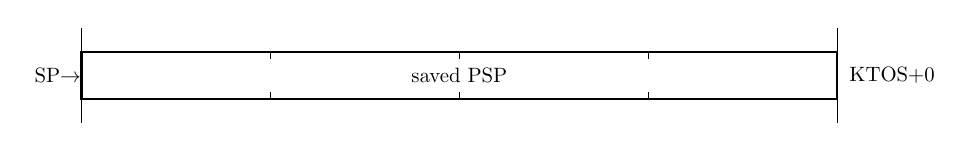
\begin{tikzpicture}[scale=0.6, every node/.style={scale=0.75}]
\draw[thick] (0,3) rectangle ++(16,1); \node at (8,3.5) {saved PSP};
\foreach \x in {4,8,12} { \draw (\x,3) -- ++(0,.15);  \draw (\x,4) -- ++(0,-.15); }
\foreach \x in {0,16} \draw (\x,2.5) -- (\x,4.5);
\node at (-.5,3.5) {SP$\rightarrow$};
\foreach \y/\offset in {3.5/0} \node[anchor=west] at (16.1,\y) {KTOS+\offset};
\end{tikzpicture}
\end{center}

Init the \lstinline{NEED_SWITCH}/\lstinline{SAVE} in \lstinline{tpl_kern}.

\begin{lstlisting}[backgroundcolor=\color{red!15}]
    mov   #tpl_kern, r11
    mov.b #NO_NEED_SWITCH_NOR_SCHEDULE, TPL_KERN_OFFSET_NEED_SWITCH(r11)
    mov.b #NO_NEED_SWITCH_NOR_SCHEDULE, TPL_KERN_OFFSET_NEED_SCHEDULE(r11)
\end{lstlisting}

Call the service. The reentrancy flag is incremented before and decremented after.
 
\begin{lstlisting}[backgroundcolor=\color{red!15}]
    inc.b &tpl_reentrancy_flag           /* surround the call by inc ...  */
    rla   REG_SID                        /* index -> offset               */
    call  tpl_dispatch_table(REG_SID)
    dec.b &tpl_reentrancy_flag           /* ... and dec of the flag.      */
\end{lstlisting}

From there, \lstinline{REG_RETARG} holds the return value. It is put at its location in the process stack. Also \lstinline{r13} and \lstinline{r14} become usable whatever is the ABI.

\begin{lstlisting}[backgroundcolor=\color{red!15}]
    pop  r13                                /* get back PSP => r13.       */
    mov  REG_RETARG, REG_RETARG_OFFSET(r13) /* put in Process's stack     */
\end{lstlisting}

Check the context switch condition in \lstinline{tpl_kern}.

\begin{lstlisting}[backgroundcolor=\color{red!15}]
    mov     #tpl_kern, r11
    tst.b   TPL_KERN_OFFSET_NEED_SWITCH(r11)
    jz      tpl_sc_handler_no_context_switch
\end{lstlisting}

\subsubsection{Branch of context switching}

Prepare the call to \lstinline{tpl_run_elected} by setting \lstinline{REG_RETARG} to 0, aka no save.
\begin{lstlisting}[backgroundcolor=\color{red!15}]
    mov     #0, REG_RETARG
\end{lstlisting}

Test the \lstinline{NEED_SAVE} condition.

\begin{lstlisting}[backgroundcolor=\color{red!15}]
    bit.b   #NEED_SAVE, TPL_KERN_OFFSET_NEED_SWITCH(r11)
    jz      tpl_sc_handler_no_save_running_context
\end{lstlisting}
Save the context. The MSP430 have a ``push multiple words", but no ``move multiple word". So, we get back to process stack to benefit this instruction

\begin{lstlisting}[backgroundcolor=\color{red!15}]
    mov     r1, r14     /* get a copy of the KSP to restore it later */
    mov     r13, r1     /* change stack to process stack */	
\end{lstlisting}
\vspace{-1em}
\begin{lstlisting}[backgroundcolor=\color{yellow!15}]
    pushm.w #7, r10     /* Push r4 to r10 on process stack (save) */
\end{lstlisting}

%\textbf{The stack pointer has been changed ! r13 IS NOT UP TO DATE !}

The whole context is now saved on process stack and the kernel stack has been cleaned. The saved context structure is shown at figure \ref{fig:context}.

\begin{figure}[h!]
\caption{Context saved on stack}
\begin{center}
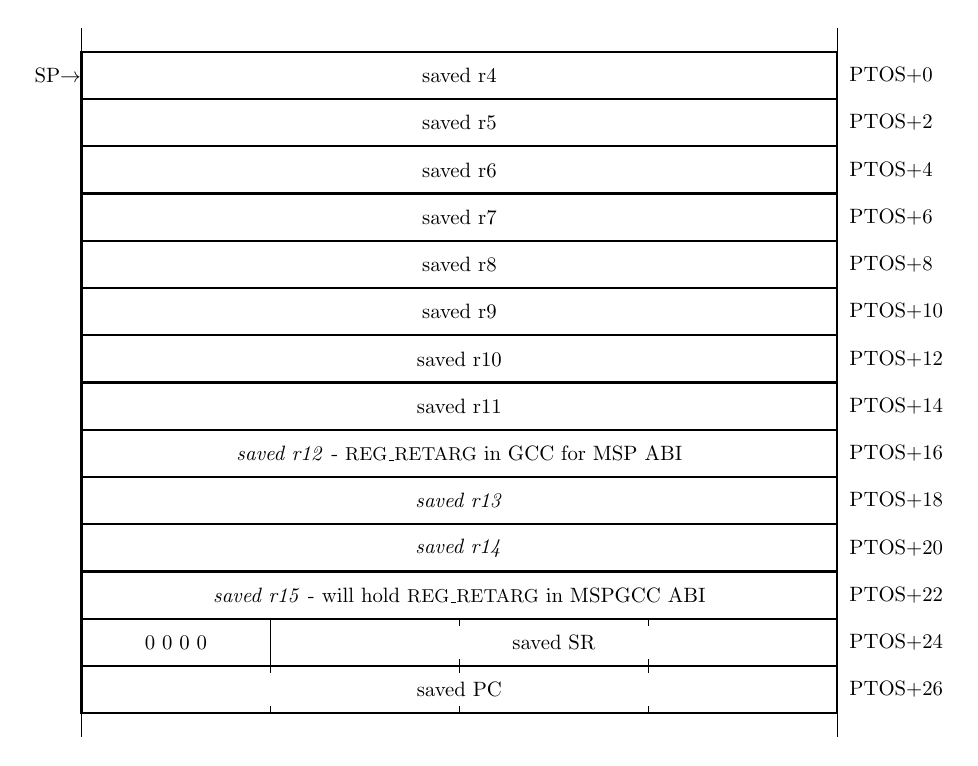
\begin{tikzpicture}[xscale=0.6, yscale=-.6, every node/.style={scale=0.75}]
\foreach \r in {4,5,...,10} {
	\draw[thick] ($(0,\r-4)$) rectangle ++(16,1); \node at ($(8,\r-4+.5)$) {saved r\r};
}
\draw[thick] (0,7) rectangle ++(16,1); \node at (8,7.5) {saved r11};
\draw[thick] (0,13) rectangle ++(16,1); \node at (8,13.5) {saved PC};
\foreach \x in {4,8,12} { \draw (\x,13) -- ++(0,.15);  \draw (\x,14) -- ++(0,-.15); }
\draw[thick] (0,12) rectangle ++(16,1); \node at (2,12.5) {0 0 0 0}; \node at (10,12.5) {saved SR};
\foreach \x in {8,12} { \draw (\x,12) -- ++(0,.15);  \draw (\x,13) -- ++(0,-.15); }
\draw (4,12) -- ++(0,1);
\draw[thick] (0,8) rectangle ++(16,1); \node at ($(8,8.5)$) {\textit{saved r12} - {\small REG\_RETARG} in GCC for MSP ABI};

\draw[thick] (0,9) rectangle ++(16,1); \node at (8,9.5) {\textit{saved r13}};
\draw[thick] (0,10) rectangle ++(16,1); \node at (8,10.5) {\textit{saved r14}};

\draw[thick] (0,11) rectangle ++(16,1); \node at ($(8,11.5)$) {\textit{saved r15} - will hold {\small REG\_RETARG} in MSPGCC ABI};
\foreach \x in {0,16} \draw (\x,-.5) -- (\x,14.5);
\node at (-.5,0.5) {SP$\rightarrow$};
\foreach \offset in {0,2,...,26} \node[anchor=west] at ($(16.1,.5+.5*\offset)$) {PTOS+\offset};
\end{tikzpicture}
\end{center}
\label{fig:context}
\end{figure}

Now the stack pointer is saved in the dedicated location.

\begin{lstlisting}[backgroundcolor=\color{yellow!15}]
    mov     &tpl_kern, r11  /* Get the s_running slot of tpl_kern in r11 */
    mov     @r11, r11       /* Get the pointer to the context (SP alone) */
    mov     r1, @r11        /* Save the stack pointer                    */
\end{lstlisting}

Prepare the argument of \lstinline{tpl_run_elected} : 1 (aka save) and call it after switching back to the kernel stack.

\begin{lstlisting}[backgroundcolor=\color{yellow!15}]
    mov     r14, r1	/* get back to kernel stack */
\end{lstlisting}
\vspace{-1em}
\begin{lstlisting}[backgroundcolor=\color{red!15}]
    mov     #1, REG_RETARG
tpl_sc_handler_no_save_running_context:
    call    tpl_run_elected
\end{lstlisting}

\lstinline{tpl_run_elected} has copied the elected process slot of \lstinline{tpl_kern} to the \lstinline{running} slot. We load the stack pointer of the new running process.

\begin{lstlisting}[backgroundcolor=\color{red!15}]
    mov     &tpl_kern, r11  /* Get the s_running slot of tpl_kern in r11 */
    mov     @r11, r11       /* Get the pointer to the context (SP alone) */
\end{lstlisting}
\begin{lstlisting}[backgroundcolor=\color{yellow!15}]
    mov     @r11, r1        /* Get the stack pointer                     */
\end{lstlisting}

Now, the context of the new running process is loaded. At start it has the same pattern as the one shown at figure \ref{fig:context}. Registers \lstinline{r4} to \lstinline{r15} are popped and we return.

\begin{lstlisting}[backgroundcolor=\color{yellow!15}]
    popm.w #12,r15       /* Pop r4 to r15 at once              */
    reti                 /* and return with interrupts enabled */
\end{lstlisting}

%\begin{figure}[h!]
%\caption{Process stack just loaded}
%\begin{center}
%\begin{tikzpicture}[scale=0.6, every node/.style={scale=0.75}]
%%\draw[thick] (0,7) rectangle ++(16,1); \node at (8,7.5) {saved r10 [15..0]};
%%\foreach \x in {4,8,12} { \draw (\x,7) -- ++(0,.15);  \draw (\x,8) -- ++(0,-.15); }
%%\draw[thick] (0,6) rectangle ++(16,1); \node at (14,6.5) {saved r10 [19..16]};
%%\draw[pattern=north west lines, pattern color=purple] (0,6) rectangle ++(12,1);
%\draw[thick] (0,13) rectangle ++(16,1); \node at (8,13.5) {saved r11 [15..0]};
%\foreach \x in {4,8,12} { \draw (\x,13) -- ++(0,.15);  \draw (\x,14) -- ++(0,-.15); }
%\draw[thick] (0,12) rectangle ++(16,1); \node at (14,12.5) {saved r11 [19..16]};
%\draw[pattern=north west lines, pattern color=purple] (0,12) rectangle ++(12,1);
%%\draw[thick] (0,3) rectangle ++(16,1); \node at (8,3.5) {saved PC [15..0]};
%%\foreach \x in {4,8,12} { \draw (\x,3) -- ++(0,.15);  \draw (\x,4) -- ++(0,-.15); }
%%\draw[thick] (0,2) rectangle ++(16,1); \node at (14,2.5) {saved PC [19..16]};
%%\draw[pattern=north west lines, pattern color=purple] (0,2) rectangle ++(12,1);
%
%\draw[thick] (0,2) rectangle ++(16,1); \node at (8,2.5) {saved PC [15..0]};
%\foreach \x in {4,8,12} { \draw (\x,3) -- ++(0,.15);  \draw (\x,4) -- ++(0,-.15); }
%\draw[thick] (0,3) rectangle ++(16,1); \node at (2,3.5) {saved PC [19..16]};
%\draw[thick] (0,3) rectangle ++(16,1); \node at (10,3.5) {saved SR [11..0]};
%\foreach \x in {4,8,12} { \draw (\x,2) -- ++(0,.15);  \draw (\x,3) -- ++(0,-.15); }
%\draw (4,3) -- ++(0,1);
%
%
%%\draw[thick] (0,1) rectangle ++(16,1); \node at (8,1.5) {service identifier};
%%\foreach \x in {4,8,12} { \draw (\x,1) -- ++(0,.15);  \draw (\x,2) -- ++(0,-.15); }
%%\draw[thick] (0,0) rectangle ++(16,1); \node at (14,.5) {saved r11 [19..16]};
%%\draw (12,0) -- ++(0,1);
%%\draw[pattern=north west lines, pattern color=purple] (0,0) rectangle ++(12,1);
%
%\foreach \y in {6,7,...,11} {
%\draw[thick] (0,\y) rectangle ++(16,1); \node at ($(8,\y+.5)$) {space of arg};
%\foreach \x in {4,8,12} { \draw (\x,\y) -- ++(0,.15);  \draw ($(\x,\y+1)$) -- ++(0,-.15); }
%}
%
%\draw[thick] (0,5) rectangle ++(16,1); \node at ($(8,5.5)$) {\small REG\_RETARG [15..0]};
%\foreach \x in {4,8,12} { \draw (\x,5) -- ++(0,.15);  \draw ($(\x,6)$) -- ++(0,-.15); }
%\draw[thick] (0,4) rectangle ++(16,1); \node at ($(14,4.5)$) {\scriptsize REG\_RETARG [19..16]};
%\draw[pattern=north west lines, pattern color=purple] (0,4) rectangle ++(12,1);
%
%\foreach \x in {0,16} \draw (\x,1.5) -- (\x,14.5);
%\node at (-.5,13.5) {SP$\rightarrow$};
%\foreach \offset in {0,2,...,22} \node[anchor=west] at ($(16.1,13.5-.5*\offset)$) {PTOS+\offset};
%\end{tikzpicture}
%\end{center}
%\label{fig:processStackLoaded}
%\end{figure}

\subsubsection{Branch of No context switching}

In case of no context switch, we have to get to the process stack, stored in r13

\begin{lstlisting}[backgroundcolor=\color{red!15}]
tpl_sc_handler_no_context_switch:
    mov  r13, r1	 /* get back to process stack */
\end{lstlisting}

Here we have the stack shaped as shown at figure \ref{fig:stackShapeBeforeCallingService}.
\lstinline{REG_RETARG} is restored, \lstinline{r11} is restored, the stack is cleaned and we return. Interrupts are enabled at that time.

\begin{lstlisting}[backgroundcolor=\color{yellow!15}]
    mov  REG_RETARG_OFFSET(r1), REG_RETARG /* get back REG_RETARG     */
    pop  r11                               /* get back r11            */
    add  #8, r1                            /* clean the stack         */
    reti                                   /* return with int enabled */
\end{lstlisting}

\subsubsection{Branch when the sc handler is called from hook}

Here we are on the kernel stack already and the \lstinline{pc} has been pushed on the stack by the \lstinline{call}. \lstinline{REG_SID} contains the identifier of the service and the 3 other registers contain the arguments if any. We do not need to do complicated stuff here because we have no context switch to do. We only call the service then return and that's it.

\begin{lstlisting}[backgroundcolor=\color{yellow!15}]
tpl_sc_handler_from_hook:
    rla   REG_SID                        /* index -> offset               */
    call  tpl_dispatch_table(REG_SID)
    ret
\end{lstlisting}

\subsection{Context initialisation}

The context that shoud be set during the task's initialisation (\lstinline{tpl_init_context}) is the one of the figure \ref{fig:context}, but with a call to either \lstinline{CallTerminateTask} or \lstinline{CallTerminateISR2} as return address of the task/ISR2 function, depending of the type of the process to init.

\begin{figure}[h!]
\caption{Context initialization}\label{fig:contextinit}
\begin{center}
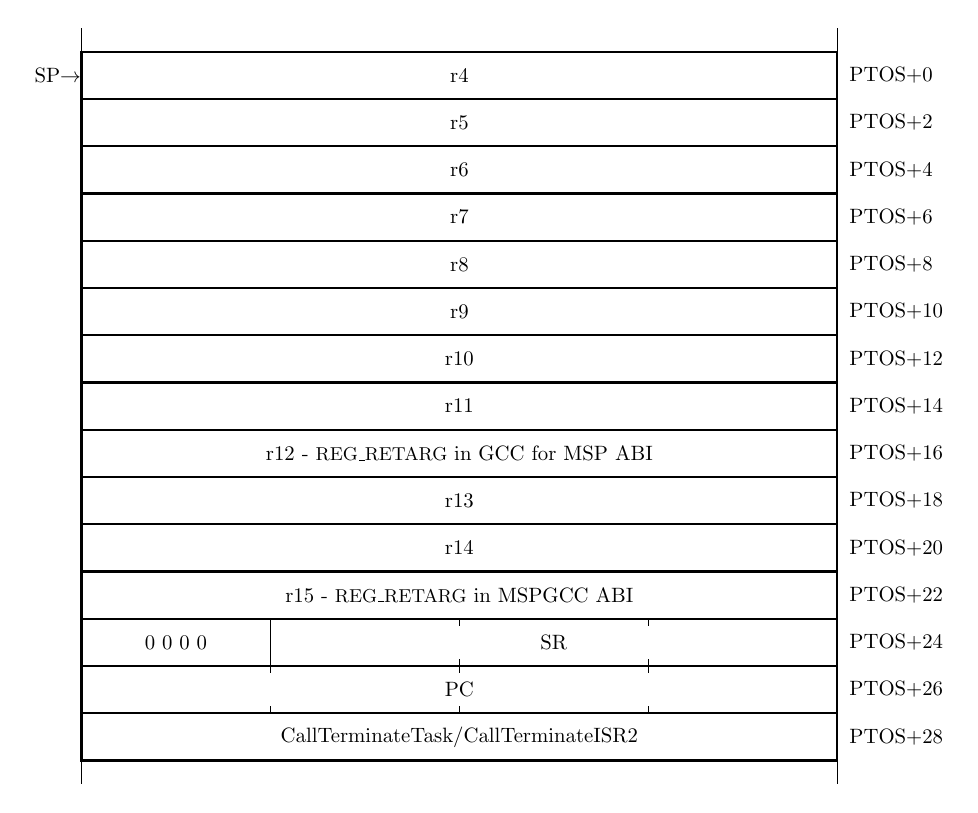
\begin{tikzpicture}[xscale=0.6, yscale=-.6, every node/.style={scale=0.75}]
\foreach \r in {4,5,...,10} {
	\draw[thick] ($(0,\r-4)$) rectangle ++(16,1); \node at ($(8,\r-4+.5)$) {r\r};
}
\draw[thick] (0,7) rectangle ++(16,1); \node at (8,7.5) {r11};
\draw[thick] (0,13) rectangle ++(16,1); \node at (8,13.5) {PC};
\foreach \x in {4,8,12} { \draw (\x,13) -- ++(0,.15);  \draw (\x,14) -- ++(0,-.15); }
\draw[thick] (0,12) rectangle ++(16,1); \node at (2,12.5) {0 0 0 0}; \node at (10,12.5) {SR};
\foreach \x in {8,12} { \draw (\x,12) -- ++(0,.15);  \draw (\x,13) -- ++(0,-.15); }
\draw (4,12) -- ++(0,1);
\draw[thick] (0,8) rectangle ++(16,1); \node at ($(8,8.5)$) {r12 - {\small REG\_RETARG} in GCC for MSP ABI};

\draw[thick] (0,9) rectangle ++(16,1); \node at (8,9.5) {r13};
\draw[thick] (0,10) rectangle ++(16,1); \node at (8,10.5) {r14};

\draw[thick] (0,11) rectangle ++(16,1); \node at ($(8,11.5)$) {r15 - {\small REG\_RETARG} in MSPGCC ABI};
\draw[thick] (0,14) rectangle ++(16,1); \node at ($(8,14.5)$) {CallTerminateTask/CallTerminateISR2};
\foreach \x in {0,16} \draw (\x,-.5) -- (\x,15.5);
\node at (-.5,0.5) {SP$\rightarrow$};
\foreach \offset in {0,2,...,28} \node[anchor=west] at ($(16.1,.5+.5*\offset)$) {PTOS+\offset};
\end{tikzpicture}


%\begin{tikzpicture}[scale=0.55, every node/.style={scale=0.75}]
%
%\foreach \reg/\y in {10/7,9/9,8/11,7/13,6/15,5/17,4/19} {
%\draw[thick] ($(0,\y+8)$) rectangle ++(16,1); \node at ($(8,\y+8.5)$) {saved r\reg [15..0]};
%\foreach \x in {4,8,12} { \draw ($(\x,\y+8)$) -- ++(0,.15);  \draw ($(\x,\y+9)$) -- ++(0,-.15); }
%\draw[thick] ($(0,\y+7)$) rectangle ++(16,1); \node at ($(14,\y+7.5)$) {saved r\reg [19..16]};
%\draw[pattern=north west lines, pattern color=purple] ($(0,\y+7)$) rectangle ++(12,1);
%}
%
%\draw[thick] (0,5) rectangle ++(16,1); \node at (8,5.5) {\small REG\_RETARG [15..0]};
%\foreach \x in {4,8,12} { \draw (\x,23) -- ++(0,.15);  \draw (\x,5) -- ++(0,-.15); }
%\draw[thick] (0,4) rectangle ++(16,1); \node at (14,4.5) {\scriptsize REG\_RETARG [19..16]};
%\draw[pattern=north west lines, pattern color=purple] (0,4) rectangle ++(12,1);
%
%
%\foreach \y in {6,7,...,11} {
%\draw[thick] (0,\y) rectangle ++(16,1); \node at ($(8,\y+.5)$) {space of arg};
%}
%
%%\draw[thick] (0,6) rectangle ++(16,1); \node at (8,6.5) {saved r15};
%%\foreach \x in {4,8,12} { \draw (\x,6) -- ++(0,.15);  \draw (\x,7) -- ++(0,-.15); }
%
%\draw[thick] (0,13) rectangle ++(16,1); \node at (8,13.5) {saved r11 [15..0]};
%\foreach \x in {4,8,12} { \draw (\x,5) -- ++(0,.15);  \draw (\x,6) -- ++(0,-.15); }
%\draw[thick] (0,12) rectangle ++(16,1); \node at (14,12.5) {saved r11 [19..16]};
%\draw[pattern=north west lines, pattern color=purple] (0,12) rectangle ++(12,1);
%
%\draw[thick] (0,2) rectangle ++(16,1); \node at (8,2.5) {saved PC [15..0]};
%\foreach \x in {4,8,12} { \draw (\x,3) -- ++(0,.15);  \draw (\x,4) -- ++(0,-.15); }
%\draw[thick] (0,3) rectangle ++(16,1); \node at (2,3.5) {saved PC [19..16]};
%\draw[thick] (0,3) rectangle ++(16,1); \node at (10,3.5) {saved SR [11..0]};
%\foreach \x in {4,8,12} { \draw (\x,2) -- ++(0,.15);  \draw (\x,3) -- ++(0,-.15); }
%\draw (4,3) -- ++(0,1);
%\foreach \x in {0,16} \draw (\x,1.5) -- (\x,28.5);
%\node at (-.5,27.5) {SP$\rightarrow$};
%\foreach \offset in {0,2,...,52} \node[anchor=west] at ($(16.1,27.5-.5*\offset)$) {PTOS+\offset};
%%22.5/0,21.5/2,20.5/4,19.5/6,18.5/8,17.5/10,16.5/12,15.5/14,14.5/16,13.5/18,
%%12.5/20,11.5/22,10.5/24,9.5/26,8.5/28,7.5/30,6.5/32,5.5/34,4.5/36,3.5/38,2.5/40,
%%1.5/42,0.5/44,-.5/46,-1.5/48,-2.5/50,-3.5/52,-4.5/54
%%} \node[anchor=west] at ($(16.1,\y+7)$) {PTOS+\offset};
%\draw[thick] (0,1) rectangle ++(16,1); \node at (8,1.5) {CallTerminateXXX [15..0]};
%\foreach \x in {4,8,12} { \draw (\x,1) -- ++(0,.15);  \draw (\x,2) -- ++(0,-.15); }
%\end{tikzpicture}
\end{center}
\label{fig:contextInit}
\end{figure}



Beside that, registers from \lstinline{r4} to \lstinline{r15} may be initialized to 0 or left uninitialized to save both execution time and energy consumption. \lstinline{PC} has to be initialized to the address of the task/ISR2 function. \lstinline{SR} has to be initialized with:
\begin{itemize}
\item \lstinline{V} at 0
\item \lstinline{SCG1}, \lstinline{SCG0}, \lstinline{OSCOFF} and \lstinline{CPUOFF} control the low power mode and are all at 0. This correspond to the Active Mode.
\item \lstinline{GIE} at 1 so interrupts are enabled when the task runs.
\item \lstinline{N}, \lstinline{Z} and \lstinline{C} at 0.
\end{itemize}

So the initialization value of \lstinline{SR} is \lstinline{0x0008}. 


\section{Interrupt Handlers}

Interrupt handlers are generated from the OIL description.
There are 3 categories of interrupt handlers in Trampoline which are handlers that link an interrupt vector to:
\begin{itemize}[noitemsep,topsep=.25em]
\item  the increment of one or more counters
\item  the execution of a category 1 ISR
\item  the execution of a category 2 ISR
\end{itemize}

The incrementation of a counter or the execution of a category 2 ISR involves an interaction with the OS with possible rescheduling and context switch, while the execution of a category 1 ISR does not involve an interaction with the OS.

For ISR 1 the interrupt handler will only backup the volatile registers, call the function implementing ISR 1 and restore the volatile registers. For ISR2 and counters, the handler will be similar to the one of the service call.

In addition, the interrupt vectors related to the GPIO ports, one vector for each port, are shared among the I/O pins of the port.

Interrupt vectors are defined in \lstinline{templates/config/msp430x/small/msp430fr5969/config.oil} file. The following vectors are available and can be used as \lstinline{SOURCE} attribute is \lstinline{ISR} and \lstinline{COUNTER} objects:

\begin{itemize}[noitemsep]
\item \lstinline{AES256_VECTOR},
\item \lstinline{RTC_VECTOR},
\item \lstinline{PORT4_VECTOR},
\item \lstinline{PORT3_VECTOR},
\item \lstinline{TIMER3_A1_VECTOR},
\item \lstinline{TIMER3_A0_VECTOR},
\item \lstinline{PORT2_VECTOR},
\item \lstinline{TIMER2_A1_VECTOR},
\item \lstinline{TIMER2_A0_VECTOR},
\item \lstinline{PORT1_VECTOR},
\item \lstinline{TIMER1_A1_VECTOR},
\item \lstinline{TIMER1_A0_VECTOR},
\item \lstinline{DMA_VECTOR},
\item \lstinline{USCI_A1_VECTOR},
\item \lstinline{TIMER0_A1_VECTOR},
\item \lstinline{TIMER0_A0_VECTOR},
\item \lstinline{ADC12_VECTOR},
\item \lstinline{USCI_B0_VECTOR},
\item \lstinline{USCI_A0_VECTOR},
\item \lstinline{WDT_VECTOR},
\item \lstinline{TIMER0_B1_VECTOR},
\item \lstinline{TIMER0_B0_VECTOR},
\item \lstinline{COMP_E_VECTOR},
\item \lstinline{UNMI_VECTOR}
\end{itemize}

Several \lstinline{ISR} or \lstinline{COUNTER} objects cannot share the same \lstinline{SOURCE}.

The \lstinline{SystemCounter} uses the \lstinline{TIMER3_A0_VECTOR} and is defined as follow in \lstinline[breaklines=true]{templates/config/msp430x/small/msp430fr5969/config.oil} file:

\begin{lstlisting}
  COUNTER SystemCounter {
    SOURCE = TIMER3_A0_VECTOR;
  };
\end{lstlisting}

When a \lstinline{PORTx_VECTOR} source is used, a \lstinline{BIT} sub-attribute can be added to select which bit is used as interrupt source. In this case several \lstinline{ISR} or \lstinline{COUNTER} may share the same vector but shall be of the same type. In other words 2 counters may share the same port vector, each on its bit or 2 ISR 1or 2 ISR 2 but you can't have a counter and an ISR sharing the same port vector or an ISR 1 and an ISR 2.

Examples can be found in \lstinline[breaklines=true]{examples/msp430x/small/msp430fr5969/launchpad}. In \lstinline{readbutton_} \lstinline{isr1}, an ISR 1 is linked to button S1 which is connected to bit \lstinline{5} of \lstinline{PORT4}:

\begin{lstlisting}
  ISR buttonS1 {
    CATEGORY = 1;
    PRIORITY = 1;
    SOURCE = PORT4_VECTOR {
      BIT = 5;
    }; /* Button S1 is on GPIO port 4, bit 5 */
  };
\end{lstlisting}

\lstinline{readbutton_isr2} is the same example but with an ISR 2 instead of the ISR 1.

\subsection{Vector table generation}

The OIL compiler generates the vector table according to what \lstinline{SOURCE} are used in the OIL file. For instance here is the vector table generated for \lstinline[breaklines=true]{readbutton_isr1} example:


\begin{lstlisting}[basicstyle=\fontsize{7.5}{9}\selectfont\ttfamily]
__attribute__ ((section(".isr_vector")))
CONST(tpl_it_handler, AUTOMATIC) tpl_it_vectors[26] = {

  /* 0xFFCC, AES256_VECTOR    */ (tpl_it_handler)tpl_null_it,
  /* 0xFFCE, RTC_VECTOR       */ (tpl_it_handler)tpl_null_it,
  /* 0xFFD0, PORT4_VECTOR     */ (tpl_it_handler)tpl_direct_irq_handler_PORT4_VECTOR,
  /* 0xFFD2, PORT3_VECTOR     */ (tpl_it_handler)tpl_null_it,
  /* 0xFFD4, TIMER3_A1_VECTOR */ (tpl_it_handler)tpl_null_it,
  /* 0xFFD6, TIMER3_A0_VECTOR */ (tpl_it_handler)tpl_primary_irq_handler_TIMER3_A0_VECTOR,
  /* 0xFFD8, PORT2_VECTOR     */ (tpl_it_handler)tpl_null_it,
  /* 0xFFDA, TIMER2_A1_VECTOR */ (tpl_it_handler)tpl_null_it,
  /* 0xFFDC, TIMER2_A0_VECTOR */ (tpl_it_handler)tpl_null_it,
  /* 0xFFDE, PORT1_VECTOR     */ (tpl_it_handler)tpl_null_it,
  /* 0xFFE0, TIMER1_A1_VECTOR */ (tpl_it_handler)tpl_null_it,
  /* 0xFFE2, TIMER1_A0_VECTOR */ (tpl_it_handler)tpl_null_it,
  /* 0xFFE4, DMA_VECTOR       */ (tpl_it_handler)tpl_null_it,
  /* 0xFFE6, USCI_A1_VECTOR   */ (tpl_it_handler)tpl_null_it,
  /* 0xFFE8, TIMER0_A1_VECTOR */ (tpl_it_handler)tpl_null_it,
  /* 0xFFEA, TIMER0_A0_VECTOR */ (tpl_it_handler)tpl_null_it,
  /* 0xFFEC, ADC12_VECTOR     */ (tpl_it_handler)tpl_null_it,
  /* 0xFFEE, USCI_B0_VECTOR   */ (tpl_it_handler)tpl_null_it,
  /* 0xFFF0, USCI_A0_VECTOR   */ (tpl_it_handler)tpl_null_it,
  /* 0xFFF2, WDT_VECTOR       */ (tpl_it_handler)tpl_null_it,
  /* 0xFFF4, TIMER0_B1_VECTOR */ (tpl_it_handler)tpl_null_it,
  /* 0xFFF6, TIMER0_B0_VECTOR */ (tpl_it_handler)tpl_null_it,
  /* 0xFFF8, COMP_E_VECTOR    */ (tpl_it_handler)tpl_null_it,
  /* 0xFFFA, UNMI_VECTOR      */ (tpl_it_handler)tpl_null_it,
  /* 0xFFFC, SYSNMI_VECTOR    */ (tpl_it_handler)tpl_MPU_violation,
  /* 0xFFFE, RESET_VECTOR     */ (tpl_it_handler)tpl_reset_handler
};
\end{lstlisting}

Obviously the last 2 vectors, \lstinline{SYSNMI_VECTOR} and \lstinline{RESET_VECTOR}, are not usable by the application and are reserved to Trampoline.

\subsection{ISR 1 interrupt handler}

An ISR 1 handler has a name formed from the concatenation of \lstinline{tpl_direct_irq_handler_} and the name of the source. For instance an ISR 1 handler for the \lstinline{PORT4_VECTOR} has the name \lstinline{tpl_direct_irq_handler_PORT4_VECTOR}.

When entering the ISR, the stack is as shown at figure \ref{fig:stackit} and \lstinline{PC} (\lstinline{r0}) and \lstinline{SR} (\lstinline{r2}) have been saved. Before doing anything we have to save the volatile registers, which are \lstinline{r11}\footnote{r11 is not volatile in the \emph{MSPGCC} ABI but is volatile in \emph{GCC compiler for MSP} ABI. Anyway, in order to limit variabilility, \lstinline{r11} is saved for both ABIs.} to \lstinline{r15}.

\begin{lstlisting}[basicstyle=\footnotesize\ttfamily]
tpl_direct_irq_handler_PORT4_VECTOR:
  pushm.w #5, r15  /* Push r11, r12, r13, r14 and r15 */
\end{lstlisting}

As a result the stack is as follow:

\begin{center}
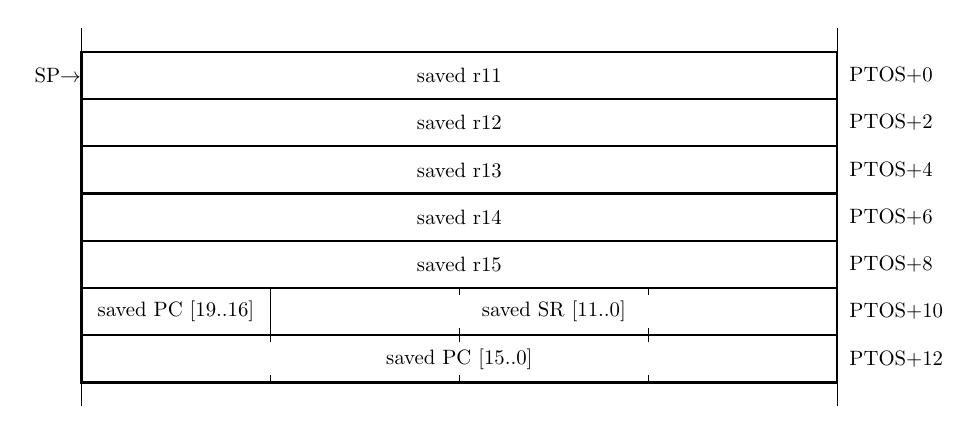
\begin{tikzpicture}[xscale=0.6, yscale=-.6, every node/.style={scale=0.75}]
\draw[thick] (0,0) rectangle ++(16,1); \node at (8,0.5) {saved r11};
\draw[thick] (0,6) rectangle ++(16,1); \node at (8,6.5) {saved PC [15..0]};
\draw[thick] (0,5) rectangle ++(16,1); \node at (10,5.5) {saved SR [11..0]}; \node at (2,5.5) {saved PC [19..16]};
\draw (4,5) -- ++(0,1);
\foreach \y in {5,6} {
	\foreach \x in {4,8,12} { \draw (\x,\y) -- ++(0,.15);  \draw ($(\x,\y+1)$) -- ++(0,-.15); }
}
%\draw[thick] (0,5) rectangle ++(16,1); \node at (8,5.5) {saved PC [15..0]};
%\foreach \x in {4,8,12} { \draw (\x,6) -- ++(0,.15);  \draw (\x,7) -- ++(0,-.15); }
%\draw[thick] (0,6) rectangle ++(16,1); \node at (14,6.5) {saved PC [19..16]};% \node at (10,5.5) {saved SR [11..0]};
%\draw[pattern=north west lines, pattern color=purple] (0,6) rectangle ++(12,1);
%\foreach \x in {4,8,12} { \draw (\x,5) -- ++(0,.15);  \draw (\x,6) -- ++(0,-.15); }
%\draw (12,6) -- ++(0,1);
\draw[thick] (0,2) rectangle ++(16,1); \node at (8,2.5) {saved r13};
\draw[thick] (0,3) rectangle ++(16,1); \node at (8,3.5) {saved r14};
\draw[thick] (0,1) rectangle ++(16,1); \node at (8,1.5) {saved r12};
\draw[thick] (0,4) rectangle ++(16,1); \node at (8,4.5) {saved r15};
\foreach \x in {0,16} \draw (\x,-.5) -- (\x,7.5);
\node at (-.5,0.5) {SP$\rightarrow$};
\foreach \offset in {0,2,...,12} \node[anchor=west] at ($(16.1,.5+.5*\offset)$) {PTOS+\offset};
\end{tikzpicture}
\end{center}

If the vector is not a port vector, the code is straightforward.

\begin{lstlisting}[basicstyle=\footnotesize\ttfamily]
  call      #buttonS1_function
\end{lstlisting}

If the vector is a port vector but no bit is specified, the ack of the interrupt is added.

\begin{lstlisting}[basicstyle=\footnotesize\ttfamily]
  call      #buttonS1_function
  mov       #0,__P4IV
\end{lstlisting}

If the vector is a port vector and a bit is specified, the generated code follows the Texas Instruments recommendations as outlined in section 12.2.6.1 of \cite{slau367o}.

\begin{lstlisting}[basicstyle=\footnotesize\ttfamily]
  add       &__P4IV, pc
  jmp       tpl_direct_irq_handler_exit_PORT4_VECTOR
  jmp       tpl_direct_irq_handler_exit_PORT4_VECTOR       /* bit 0 */
  jmp       tpl_direct_irq_handler_exit_PORT4_VECTOR       /* bit 1 */ 
  jmp       tpl_direct_irq_handler_exit_PORT4_VECTOR       /* bit 2 */
  jmp       tpl_direct_irq_handler_exit_PORT4_VECTOR       /* bit 3 */
  jmp       tpl_direct_irq_handler_exit_PORT4_VECTOR       /* bit 4 */
  jmp       tpl_p4_5_handler                               /* bit 5 */
  jmp       tpl_direct_irq_handler_exit_PORT4_VECTOR       /* bit 6 */
  jmp       tpl_direct_irq_handler_exit_PORT4_VECTOR       /* bit 7 */
tpl_p4_5_handler:
  call      #buttonS1_function
tpl_direct_irq_handler_exit_PORT4_VECTOR:
\end{lstlisting}

Then the volatile registers are restored and we return.

\begin{lstlisting}[basicstyle=\footnotesize\ttfamily]
  popm.w    #5, r15
  reti
\end{lstlisting}

\subsection{ISR 2 interrupt handler}

An ISR 2 handler has a name formed from the concatenation of \lstinline{tpl_primary_irq_handler_} and the name of the source. For instance an ISR 2 handler for the \lstinline{PORT4_VECTOR} has the name \lstinline{tpl_primary_irq_handler_PORT4_VECTOR}.

When entering the ISR, the stack is as shown at figure \ref{fig:stackit} and \lstinline{PC} (\lstinline{r0}) and \lstinline{SR} (\lstinline{r2}) have been saved. Before doing anything we have to save the volatile registers, which are \lstinline{r11} to \lstinline{r15}.

\begin{lstlisting}[basicstyle=\footnotesize\ttfamily]
tpl_primary_irq_handler_PORT4_VECTOR:
  pushm.w #5, r15  /* Push r11, r12, r13, r14 and r15 */
\end{lstlisting}

Then we switch to the kernel stack and init \lstinline{tpl_kern}.

\begin{lstlisting}[basicstyle=\footnotesize\ttfamily]
  mov       r1, r11                         /* Copy the PSP in r11      */
  mov       #tpl_kern_stack + TPL_KERNEL_STACK_SIZE, r1 /* kernel stack */
  push      r11                             /* Save PSP to kernel stack */
  mov       #tpl_kern, r11
  mov.b     #NO_NEED_SWITCH_NOR_SCHEDULE, TPL_KERN_OFFSET_NEED_SWITCH(r11)
  mov.b     #NO_NEED_SWITCH_NOR_SCHEDULE, TPL_KERN_OFFSET_NEED_SCHEDULE(r11)
\end{lstlisting}

Activate the ISR 2. Here the \lstinline{#1} in \lstinline{mov #1, REG_RETARG} is the identifier of the ISR 2. Only the most complex generated code is shown.

\begin{lstlisting}[basicstyle=\footnotesize\ttfamily]
  add       &__P4IV, pc
  jmp       tpl_direct_irq_handler_exit_PORT4_VECTOR
  jmp       tpl_direct_irq_handler_exit_PORT4_VECTOR       /* bit 0 */
  jmp       tpl_direct_irq_handler_exit_PORT4_VECTOR       /* bit 1 */
  jmp       tpl_direct_irq_handler_exit_PORT4_VECTOR       /* bit 2 */
  jmp       tpl_direct_irq_handler_exit_PORT4_VECTOR       /* bit 3 */
  jmp       tpl_direct_irq_handler_exit_PORT4_VECTOR       /* bit 4 */
  jmp       tpl_p4_5_handler                               /* bit 5 */
  jmp       tpl_direct_irq_handler_exit_PORT4_VECTOR       /* bit 6 */
  jmp       tpl_direct_irq_handler_exit_PORT4_VECTOR       /* bit 7 */
tpl_p4_5_handler:
  mov       #1, REG_RETARG
  call      #tpl_fast_central_interrupt_handler
\end{lstlisting}

The remaining code is similar to the one of the \lstinline{tpl_sc_handler}.

\begin{lstlisting}[basicstyle=\footnotesize\ttfamily]
tpl_direct_irq_handler_exit_PORT4_VECTOR:
  mov       r1, r13 /* get a copy of the KSP to restore it later        */
  add       #2, r13 /* and forget the pushed PSP (not useful anymore).  */
  pop       r1      /* get the saved process stack pointer back         */
  mov       #tpl_kern, r11
  tst.b     TPL_KERN_OFFSET_NEED_SWITCH(r11)
  jz        tpl_PORT4_VECTOR_no_context_switch
  pushm.w   #7, r10  /* Push r4 to r10 */
  mov       &tpl_kern, r11 /* Get the s_running slot of tpl_kern in r11 */
  mov       @r11, r11      /* Get the pointer to the context (SP alone) */
  mov       r1, @r11       /* Save the stack pointer                    */
  mov       r13, r1        /* Switch back to the kernel stack           */
  mov       #1, REG_RETARG
  call      #tpl_run_elected
  mov       &tpl_kern, r11 /* Get the s_running slot of tpl_kern in r11 */
  mov       @r11, r11      /* Get the pointer to the context (SP alone) */
  mov       @r11, r1       /* Get the stack pointer                     */
  popm.w    #12,r15        /* Pop r4 to r15  */
  reti
tpl_PORT4_VECTOR_no_context_switch:
  popm.w    #5, r15
  reti
\end{lstlisting}

\subsection{Counter interrupt handler}

A counter interruption handler has the same structure as that of an ISR 2. The only difference is the function called. For instance for the SystemCounter the code is straightforward.

\begin{lstlisting}[basicstyle=\footnotesize\ttfamily]
tpl_primary_irq_handler_TIMER3_A0_VECTOR:

/*--------------------------------------------------------------------------
 * -1- Before doing anything we have to save the volatile registers, which
 * are r11 (r11 is not volatile in the MSPGCC ABI but is volatile in GCC
 * compiler for MSP ABI. Anyway, in order to limit variabilility, r11 is 
 * saved for both ABIs) to r15, because they will not be saved when we will
 * call the underlying C function.
 */
  pushm.w   #5, r15  /* Push r11, r12, r13, r14 and r15 */
/*--------------------------------------------------------------------------
 * -2- Switch to the kernel stack.
 */
  mov       r1, r11                          /* Copy the PSP in r11      */
  mov       #tpl_kern_stack + TPL_KERNEL_STACK_SIZE, r1 /* kernel stack  */
  push      r11                              /* Save PSP to kernel stack */
/*--------------------------------------------------------------------------
 * -3- Init the NEED_SWITCH/SAVE in tpl_kern.
 */
  mov       #tpl_kern, r11
  mov.b     #NO_NEED_SWITCH_NOR_SCHEDULE, TPL_KERN_OFFSET_NEED_SWITCH(r11)
  mov.b     #NO_NEED_SWITCH_NOR_SCHEDULE, TPL_KERN_OFFSET_NEED_SCHEDULE(r11)
/*--------------------------------------------------------------------------
 * -4- Call the underlying C function.
 */
  call      #tpl_tick_TIMER3_A0_VECTOR
/*--------------------------------------------------------------------------
 * -5- Switch back to the process stack
 */
tpl_direct_irq_handler_exit_TIMER3_A0_VECTOR:
  mov       r1, r13 /* get a copy of the KSP to restore it later        */
  add       #2, r13 /* and forget the pushed PSP (not useful anymore).  */
  pop       r1      /* get the saved process stack pointer back         */
/*--------------------------------------------------------------------------
 * -6- Check the context switch condition in tpl_kern.
 */
  mov       #tpl_kern, r11
  tst.b     TPL_KERN_OFFSET_NEED_SWITCH(r11)
  jz        tpl_TIMER3_A0_VECTOR_no_context_switch
/*--------------------------------------------------------------------------
 * -7- Save the rest of the context.
 */ 
  pushm.w   #7, r10  /* Push r4 to r10 */
/*--------------------------------------------------------------------------
 * -8- Now the stack pointer is saved in the dedicated location.
 */  
  mov       &tpl_kern, r11 /* Get the s_running slot of tpl_kern in r11 */
  mov       @r11, r11      /* Get the pointer to the context (SP alone) */
  mov       r1, @r11       /* Save the stack pointer                    */
/*--------------------------------------------------------------------------
 * -9- Call tpl_run_elected with argument 1 (aka save) after switching back
 * to the kernel stack.
 */
  mov       r13, r1        /* Switch back to the kernel stack           */
  mov       #1, REG_RETARG
  call      #tpl_run_elected
/*--------------------------------------------------------------------------
 * -10- tpl_run_elected has copied the elected process slot of tpl_kern to
 * the running slot. We load the stack pointer of the new running process.
 */
  mov       &tpl_kern, r11 /* Get the s_running slot of tpl_kern in r11 */
  mov       @r11, r11      /* Get the pointer to the context (SP alone) */
  mov       @r11, r1       /* Get the stack pointer                     */
/*--------------------------------------------------------------------------
 * -11- Now, the context of the new running process is loaded. All registers
 * are popped.
 */
  popm.w    #12,r15        /* Pop r4 to r15  */
  reti
/*--------------------------------------------------------------------------
 * -12- We get here from stage 6. Restore the volatile registers and return
 * from the interrupt handler.
 */
tpl_TIMER3_A0_VECTOR_no_context_switch:
  popm.w    #5, r15
  reti
\end{lstlisting}

\section{MCU Clocks}
The MCU clocks uses the DCO as input clock. The CPU is limited to 16MHz. 

\subsection{Startup}
The MCU clocks can be defined in the .oil file directly in \texttt{CPU->OS->CPU\_FREQ\_MHZ}. Value should be in the set \emph{1,2,4,6,8,12,16,21 and 24} MHz.

By default, the frequency is set to 1MHz.

\subsection{Dynamic update}
The MCU clocks can be updated with a user fonction to update the frequency in \lstinline{tpl_clocks.h}:

\begin{lstlisting}
/* configure the frequency in MHz: 1,2,4,6,8,12,16,(21,24 overclock)
 * set to 1MHz in case of bad input frequency.
 **/

FUNC(void,OS_CODE) tpl_set_mcu_clock(uint16_t freq);
\end{lstlisting}

When the CPU clock is updated, the Wait States for the FRAM access are set accordingly: 1 wait state above 8MHz, and 2 wait states above 16MHz.

Note that the 21MHz and 24 MHz frequencies overclock the CPU capabilities and may not work.

A callback can be added each time the CPU clock is updated. This is done through the function:
\begin{lstlisting}
void tpl_add_freq_update_callback(tpl_freq_update_item *freqObs);
\end{lstlisting}
Where \lstinline{freqObs} is an item of a single linked list of function calls. This functionnality is implemented in the serial line driver (for debug purpose) of the launchpad like this:

\begin{lstlisting}
#include "tpl_clocks.h"

tpl_freq_update_item tpl_serial_callback = {&tpl_serial_update_freq,NULL};

void tpl_serial_begin()
{
	/* make sure we are informed of a clock update. */
	tpl_add_freq_update_callback(&tpl_serial_callback);
	..
}

void tpl_serial_update_freq()
{
	//callback that updates the serial baudrate configuration
	//in function of the new input clock.
}

\end{lstlisting}

The frequency of the MCU is defined using the DCO. The function \lstinline{uint32_t tpl_getDCOFrequency();} returns the DCO output frequency in Hz. This can be used in the function callback.


\section{Low power in idle}

When Trampoline runs the idle task, the MCU can be put in low power mode. This is done by setting the attribute \lstinline{IDLE_POWER_MODE} in the \lstinline{OS} object. Possible values are \lstinline{ACTIVE}, \lstinline{LPM0}, \lstinline{LPM1}, \lstinline{LPM2} and \lstinline{LPM3}. Default value, that is without setting this attribute, is \lstinline{ACTIVE}.

\section{Stack size estimation}

In the following, tasks and ISR2s are collectively referred to as processes. Stack size of a process depends on what function the process calls, the size of the local variables, the optimization level of the compiler and if at least one ISR1 is used by the application\footnote{ISR1 executes on the stack of the running task/ISR2}. So it is not something that is easy to compute. The minimum stack size of a process is the size needed to store an initialized context as shown at figure \ref{fig:contextinit}, i.e. 30 bytes.

When the process runs, the context is popped and the only element left on the stack is the return address to \lstinline{CallTerminateTask} or \lstinline{CallTerminateISR2}, which leaves 28 bytes for local variables and function calls.

Calling an OS service requires 14 bytes if the service does not lead to a context save and 28 bytes if it does not. Since the kernel runs on a dedicated stack, the stack depth required to run a service has no impact on the stack size of a process.

\subsection*{Example of a trivial basic task}

Let's take the blink task from the example \lstinline{readbutton_isr2}. Once compiled in \lstinline{-O0}, the generated code is as follow:

\begin{lstlisting}[basicstyle=\footnotesize\ttfamily]
00006238 <blink_function>:
    6238:       04 12           push    r4              
    623a:       04 41           mov     r1,     r4      
    623c:       24 53           incd    r4              
    623e:       5f 42 02 02     mov.b   &0x0202,r15         /* read port  */
    6242:       6f e3           xor.b   #2,     r15         /* toggle     */
    6244:       c2 4f 02 02     mov.b   r15,    &0x0202     /* write port */
    6248:       b0 12 54 61     call    #0x6154     /* Call TerminateTask */
    624c:       34 41           pop     r4              
    624e:       30 41           ret                     
\end{lstlisting}

By pushing \lstinline{r4} on the stack and calling \lstinline{TerminateTask}, the amount of stack consumed is 16 bytes out of the 28 bytes available. The minimum stack size is therefore sufficient. However, pressing the button at the time the task is executed leads to its pre-emption and the execution of ISR2. In this case, the stack must be able to contain the register \lstinline{r4} that has been pushed and the context of the task, namely 30 bytes. By adding the two bytes of the \lstinline{CallTerminateTask} address, the minimum stack is 32 bytes.

When the application is compiled in \lstinline{-O3}, the blink task code is as follows:

\begin{lstlisting}[basicstyle=\footnotesize\ttfamily]
00005d60 <blink_function>:
    5d60:       e2 e3 02 02     xor.b   #2,     &0x0202     /* toggle     */
    5d64:       b0 12 7a 5c     call    #0x5c7a     /* Call TerminateTask */ 
    5d68:       30 41           ret                     
\end{lstlisting}

This time \lstinline{r4} is not pushed on the stack and its size can be 30 bytes. Given the time taken to complete this task, it is also questionable whether it would not be worthwhile to make it non-preemptible.

\section{Using the DMA to copy the initialized variable}

It is possible to copy the initialized variable by using the DMA. This is done by adding a \lstinline{INIT_WITH_DMA = TRUE;} in the OS object.

\section{Memory mapping and memory protection}

Memory organization of MSP430FR5969 is shown at figure \ref{fig:memorg}. 

\begin{figure}[htbp] %  figure placement: here, top, bottom, or page
\centering
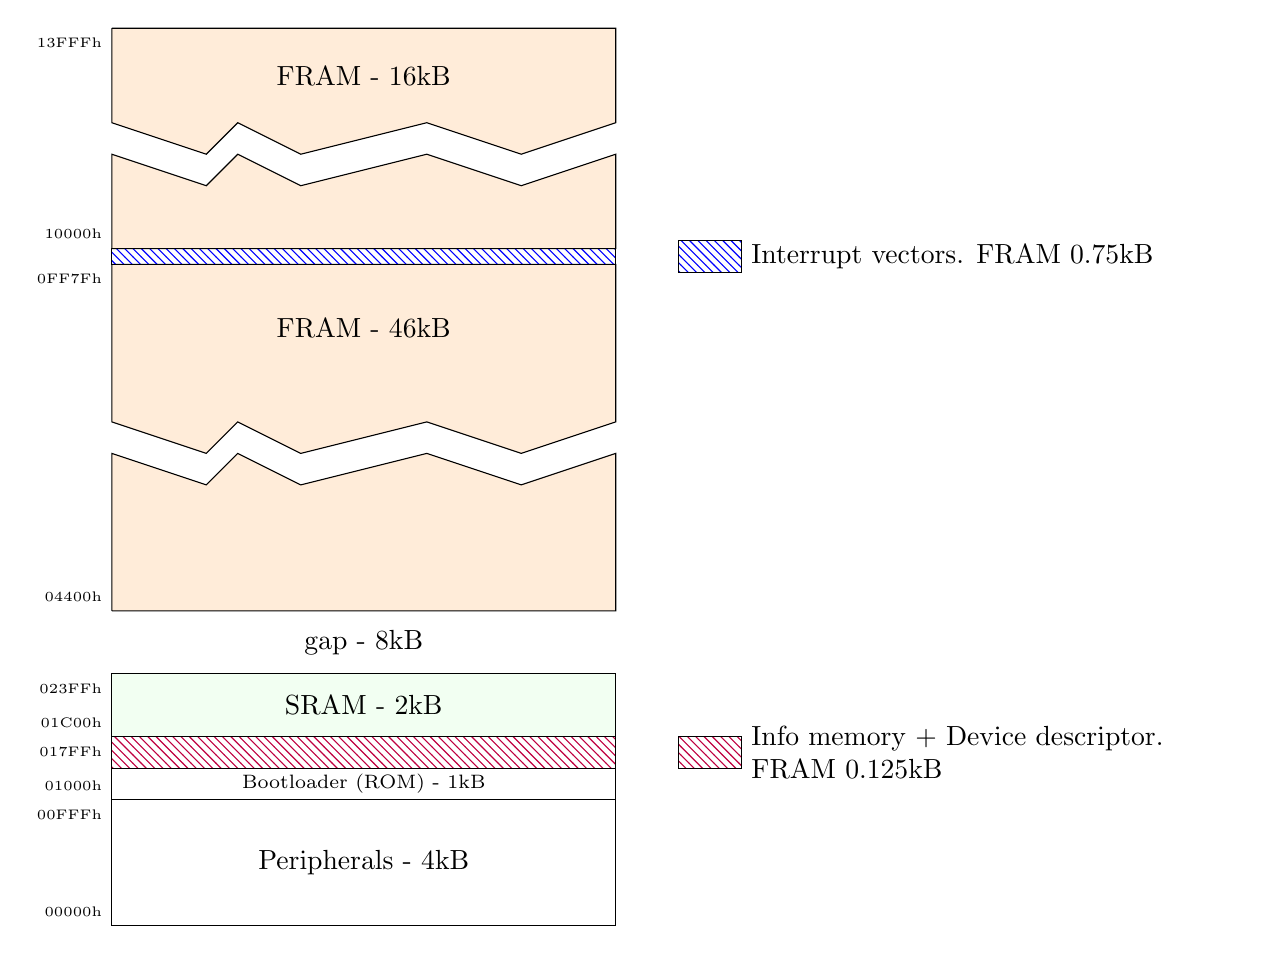
\begin{tikzpicture}[scale=0.4, every node/.style={scale=1}]
\draw (0,0) rectangle ++(16,4); \node at (8,2) {Peripherals - 4kB}; \node[anchor=south east] at (0,0) {\tiny 00000h}; \node[anchor=north east] at (0,4) {\tiny 00FFFh};
\draw (0,4) rectangle ++(16,1); \node at (8,4.5) {\scriptsize Bootloader (ROM) - 1kB}; \node[anchor=south east] at (0,4) {\tiny 01000h}; \node[anchor=north east] at (0,6) {\tiny 017FFh};
\draw[pattern=north west lines, pattern color=purple] (0,5) rectangle ++(16,1);
\draw[fill=green!5] (0,6) rectangle ++(16,2); \node at (8,7) {SRAM - 2kB}; \node[anchor=south east] at (0,6) {\tiny 01C00h}; \node[anchor=north east] at (0,8) {\tiny 023FFh};
%\draw (0,6) rectangle ++(16,.5); \node[anchor=north west] at (16.1,6.25) {Information (FRAM) - .5kB}; %\node[anchor=south east] at (0,6) {\tiny 01800h}; \node[anchor=north east] at (0,6.5) {\tiny 019FFh};
%\draw (0,6.5) rectangle ++(16,.25); \node[anchor=south west] at (16.1,6.625) {Dev. Desc. (FRAM) - .25kB}; %\node[anchor=south east] at (0,6) {\tiny 01800h}; \node[anchor=north east] at (0,6.5) {\tiny 019FFh};
\node at (8,9) {gap - 8kB};
\draw[fill=orange!15] (0,10) -- ++(16,0) -- ++(0,5) -- ++(-3,-1) -- ++(-3,1) -- ++ (-4,-1) -- ++(-2,1) -- ++(-1,-1) -- ++(-3,1) -- ++(0,-5);
\draw[fill=orange!15] (0,21) -- ++(16,0) -- ++(0,-5) -- ++(-3,-1) -- ++(-3,1) -- ++ (-4,-1) -- ++(-2,1) -- ++(-1,-1) -- ++(-3,1) -- ++(0,5);
\node at (8,19) {FRAM - 46kB}; \node[anchor=south east] at (0,10) {\tiny 04400h}; \node[anchor=north east] at (0,21) {\tiny 0FF7Fh};

\draw[pattern=north west lines, pattern color=blue] (0,21) rectangle ++(16,.5);

\draw[fill=orange!15] (0,21.5) -- ++(16,0) -- ++(0,3) -- ++(-3,-1) -- ++(-3,1) -- ++ (-4,-1) -- ++(-2,1) -- ++(-1,-1) -- ++(-3,1) -- ++(0,-3);
\draw[fill=orange!15] (0,28.5) -- ++(16,0) -- ++(0,-3) -- ++(-3,-1) -- ++(-3,1) -- ++ (-4,-1) -- ++(-2,1) -- ++(-1,-1) -- ++(-3,1) -- ++(0,3);
\node at (8,27) {FRAM - 16kB}; \node[anchor=south east] at (0,21.5) {\tiny 10000h}; \node[anchor=north east] at (0,28.5) {\tiny 13FFFh};

\draw[pattern=north west lines, pattern color=blue] (18,20.75) rectangle ++(2,1); \node[anchor=west] at (20,21.25) {Interrupt vectors. FRAM 0.75kB};
\draw[pattern=north west lines, pattern color=purple] (18,5) rectangle ++(2,1); \node[anchor=west,text width=6cm] at (20,5.5) {Info memory + Device descriptor. FRAM 0.125kB};
\end{tikzpicture}
\caption{Memory organization of MSP430FR5969}
\label{fig:memorg}
\end{figure}

The TI MSP430 uses a very simple memory protection scheme. The Memory Protection Unit allows to define 2 boundaries, SEGB1 and SEGB2 and the access right corresponding to 3 regions, the one below SEGB1 (excluded), the one between SEGB1 (included) and SEGB2 (excluded) and the one above SEGB2 (included). Some addresses locations, the 16 bytes starting à \lstinline{0xFF80} contain the JTAG password. Writing random values at theses addresses bricks the MCU. To prevent that, Trampoline initialize the MPU so that addresses below the start of FRAM (peripherals and SRAM) may be read and written, addresses from start of FRAM to \lstinline{0x10000} may be read and executed and addresses from \lstinline{0x10000} to the end of the FRAM may be read and written.

\section{Libraries}
\subsection{Serial line}
The launchpad kits use a serial line over USB that can be used for debugging purpose. The configuration is \emph{9600 bauds, 8N1}. The clock is the DCO, which is not precise enough to get a correct 115200 bauds communication.

The library should be declared in the .oil file (so that dedicated files are included in the build process), with 2 parameters:
\begin{lstlisting}
  BUILD = TRUE {
    LIBRARY = serial {
      TXBUFFER = 16;
      RXBUFFER = 16;
    };
  };
\end{lstlisting}

The buffers are ring buffers that are updated in the corresponding RX or TX interrupts. If the buffer size is set to 0, the corresponding interrupt is not enabled.

The library supports various MCU change frequencies, and the output frequency is updated (the current message may be corrupted!).

An example is given for the msp430fr5969 launchpad.
\bibliographystyle{plain}
\bibliography{porting}

\end{document}  
